\documentclass[a4paper,14pt]{extarticle} %размер бумаги устанавливаем А4, шрифт 12пунктов
\usepackage[T2A]{fontenc}
%\usepackage[utf8]{inputenc} 
\usepackage[utf8x]{inputenc}
\usepackage[T1]{fontenc}
\usepackage{textcomp}
\usepackage{float}
\inputencoding{utf8}
\usepackage[english,russian]{babel}%используем русский и английский языки с переносами
\usepackage{amssymb,amsfonts,amsmath,mathtext,cite,enumerate,float}%подключаем нужные пакеты расширений
\usepackage[pdftex]{graphicx} %хотим вставлять в диплом рисунки?
\graphicspath{{./images/}}
\usepackage{color}
\usepackage[ section ]{ placeins}
\usepackage[pdftex]{lscape}
\usepackage{hyperref}
\usepackage{lscape}
\usepackage{svg}
\setsvg{inkscape = inkscape -z -D}
\setsvg{svgpath = images/}
\usepackage{epstopdf}
%\graphicspath{{noiseimages/}}%путь к рисункам
\usepackage{listings}
\lstset{language=Fortran}
\makeatletter
\renewcommand{\@biblabel}[1]{#1.} % Заменяем библиографию с квадратных скобок на точку:
\makeatother
\setcounter{tocdepth}{3}
\usepackage{geometry} % Меняем поля страницы
\makeatletter
\@addtoreset{equation}{subsection}
\makeatother

\newcommand{\frp}[2]{\frac{\partial #1}{\partial #2}}

\renewcommand*{\thesection}{\arabic{section}}

\geometry{left=2cm}% левое поле
\geometry{right=1.5cm}% правое поле
\geometry{top=1cm}% верхнее поле
\geometry{bottom=2cm}% нижнее поле


\makeatletter
%\renewcommand{\@biblabel}[1]{#1.} % Заменяем библиографию с квадратных скобок на точку:
\makeatother

\usepackage{geometry} % Меняем поля страницы
\geometry{left=3cm}% левое поле
\geometry{right=1cm}% правое поле
\geometry{top=2cm}% верхнее поле
\geometry{bottom=2cm}% нижнее поле
\renewcommand*{\thesection}{\arabic{section}}

\abovedisplayskip=1.5\abovedisplayskip %отбивки вокруг формул

\renewcommand{\baselinestretch}{1.5}

\renewcommand{\theenumi}{\arabic{enumi}}% Меняем везде перечисления на цифра.цифра
\renewcommand{\labelenumi}{\arabic{enumi}}% Меняем везде перечисления на цифра.цифра
\renewcommand{\theenumii}{.\arabic{enumii}}% Меняем везде перечисления на цифра.цифра
\renewcommand{\labelenumii}{\arabic{enumi}.\arabic{enumii}.}% Меняем везде перечисления на цифра.цифра
\renewcommand{\theenumiii}{.\arabic{enumiii}}% Меняем везде перечисления на цифра.цифра
\renewcommand{\labelenumiii}{\arabic{enumi}.\arabic{enumii}.\arabic{enumiii}.}% Меняем везде перечисления на цифра.цифра

\begin{document}
\begin{titlepage}

\begin{center}
Федеральное государственное автономное образовательное\\
учреждение высшего образования\\
<<Санкт-Петербургский Политехнический университет Петра Великого>>\\
Институт физики, нанотехнологий и телекоммуникаций\\
Кафедра космических исследований \\
\end{center}  

\vspace{1em}

\begin{flushright}
\parindent=0pt
\makebox[15em][l]{Работа допущена к защите}\\
\makebox[15em][l]{Заведующий кафедрой КИ}\\
\makebox[15em][l]{\hrulefill Варшалович Д.А.}\\
\makebox[15em][l]{<<\hrulefill >>\hrulefill 2015 г.\phantom{mmmm}}
\end{flushright}

\vspace{1em}

\begin{center}
ВЫПУСКНАЯ РАБОТА БАКАЛАВРА\\
\Large\textbf{<<Численное моделирование ускорения частиц\\ на ударных волнах>>}
\end{center}

\vspace{1em}

\begin{flushleft}
\begin{tabbing}
aaaaaaaaaaaaaaaaa \= aaaaaaaaaaaaaaaaaaaaaaa \kill
Направление: \> 03.03.02 -- <<Физика>>\\
Профиль: \> <<Физика космоса>>\\
\end{tabbing}
\end{flushleft}

\vspace{1em}

\begin{tabbing}
  \hspace{17cm}\=\kill
  Студент гр.43412\>\textbf{Лиознов А.В.}\'\\~\\
  Руководитель\> \'\\
  н.с. ФТИ им.\\
А.Ф.Иоффе, к.ф.-м.н.\>\textbf{Гладилин П.Е.}\'\\
\end{tabbing}

\vspace{\fill}

\begin{center}
Санкт-Петербург\\
2015
\end{center}

\end{titlepage}
\newpage
\tableofcontents
\newpage
\section{Введение}
\subsection{Актуальность}
В течение продолжительного времени учёные пытаются определить, как образуется наблюдаемое распределение космических лучей по энергиям. Далеко не весь диапазон спектра можно описать с помощью теплового взаимодействия.

Особую роль играют механизмы нетеплового ускорения частиц в бесстолкновительной космической плазме. 

Такие частицы можно непосредственно наблюдать в межпланетном пространстве, частицы низких энергий - посредством прямых измерений  с Земли, а частицы высоких энергий ($>10^5$ ГэВ) - в виде широких атмосферных ливней.

Особый интерес составляет процесс ускорения на фронтах ударных волн, в силу их распространённости.
Примерами таких волн могут служить волны от хромосферных солнечных вспышек, вспышек сверхновых звёзд, ударные волны звёздного ветра...

Дополнительный интерес к данным процессам связан с возможностью выделения в них большого количества энергии, существенная часть которой может быть преобразована в направленное ускорение небольшого количества частиц, что и приводит к появлению частиц с энергиями, на много порядков превышающих тепловые.

Построение численных моделей ударных волн необходимо для понимания данных процессов.

Проблемой занимаются давно.\\
 Бережко Е. Г. и Крымский Г. Ф. в 1988 году привели теоретический вывод диффузиозно-конвективного уравнения. Х. Канг в 2011 году провёл численные расчёты спектров ускоренных частиц. \\ 
С другой стороны к задаче подошёли А. Ахтенберг и В. Круллс, которые в 1992 году провёли моделирование ускорения стохастическим методом.

И, хотя сравнения данных подходов предпринимались, количественные оценки как с точки зрения времени работы, так и с точки зрения простоты реализации и расширяемости сделаны не были.

\subsection{Цели и задачи}
В связи со всем вышесказанным целью работы был анализ и сравнение \\
диффузиозно-конвективного и стохастического подхода в ускорении частиц на ударных волнах.

В рамках этой цели были поставлены следующие задачи:
\begin{enumerate}
\item Реализовать численное моделирование решения диффузиозно- конвективного уравнения методом Эйлера в ускорении частиц на ударных волнах.
\item Реализовать численное моделирование ускорения частиц на ударных волнах стохастическим методом.
\item Провести сравнение данных подходов
\item Указать положительные и отрицательные стороны в каждом из них
\end{enumerate}

\subsection{Процесс ускорения на ударных волнах}
Рассмотрим физическую сторону процесса ускорения на ударных волнах:

Движение частиц плазмы определяется не соударениями, как в случае теплового движения, а взаимодействием с возникающий на фронте турбулентностью. Характерной длиной, определяющей толщину фронта, является гирорадиус тепловых ионов.

Несмотря на то, что сама теория ударных волн ещё далека от завершения, характер достаточно быстрых частиц на фронте мало зависит от особенностей структуры. Это связано с тем, что движение частиц зависит, в основном, от двух факторов: взаимодействии с магнитным полем - крупномасштабным, регулярным, с одной стороны, и турбулентным, хаотичным - с другой. Это поле приводит к рассеянию частиц, причём свободный пробег сильно превышает толщину фронта.

Возможность ускорения частиц связана, прежде всего, с имеющимися в пространстве электрическими полями. Для иллюстрации на рисунке \ref{intro/lam}а схематически изображена траектория частицы в системе покоя фронта в случае, когда мелкомасштабные электрические поля отсутствуют. Для быстрой частицы ударная волна представляет собой магнитогидродинамический разрыв, в котором скорость плазмы $u$, плотность $\rho$, магнитное поле $B$ связано следующими соотношениями:
\begin{eqnarray}
\rho_2 = \sigma \rho_1\\
u_2=\frac{u_1}{\sigma}\\
B_2=\sigma B_1
\end{eqnarray}
Где индексы 1, 2 означают область до и после фронта соответственно, а $\sigma$ - степень сжатия вещества.

Пересекая фронт, частица испытывает градиентный дрейф и смещается вдоль электрического поля
$\vec{E} = - [\vec{u}\vec{B}]/c$, где $c$ - скорость света.

\begin{figure}[htbp]
  \centering
  \includesvg[width=400px]{lamin}
  \caption{\label{intro/lam} Движение быстро заряженной частицы в ламинарной ударной волне (а) и турбулетной(б)}
\end{figure}
Каждая частица рассеивается на неоднородностях магнитного поля (рис \ref{intro/lam}б), что приводит к многократному перемещению между областями фронтов и многократному ускорению. За один цикл (двукратное пересечение фронта) среднее изменение импульса частицы будет равно
\begin{equation}
\left< \Delta p \right> = \frac{4}{3} (u_2-u_1)\frac{p}{v}
\end{equation}
Где $u_2$, $u_1$ - скорость плазмы за и перед фронтом, $v$ - скорость частицы.

В каждом цикле часть частиц уходит и уже не возвращается к фронту. Интегральный спектр ускорения частиц $N(p)$ - количество частиц в единице объёма с импульсами, большими $p$,  - может быть найден из уравнения баланса
\begin{equation}
\frac{dN}{dp}=\frac{P_c-1}{\left<\Delta p \right>}N
\end{equation}
Где $P_c$ - вероятность совершения очередного цикла. $P_c=P_1 \cdot P_2$, где $P_1$ - вероятность частицы попавшей в область перед фронтом, вернуться на фронт и равна 1, а $P_2$ - аналогичная вероятность для области за фронтом и равна $1-\frac{4u_2}{v}$

Используя последние уравнения, можно получить уравнение на плотность:
\begin{equation}
\frac{d pn}{dp} + 3 \frac{u_2}{u_1-u_2} n = 0
\end{equation}

Решением данного уравнения будет являться функция $n \sim p^{-\gamma}$ с показателем $\gamma=\frac{\sigma+2}{\sigma-1}$

\subsubsection{Ускорение на двух ударных волнах}

\begin{figure}[H]
\centering
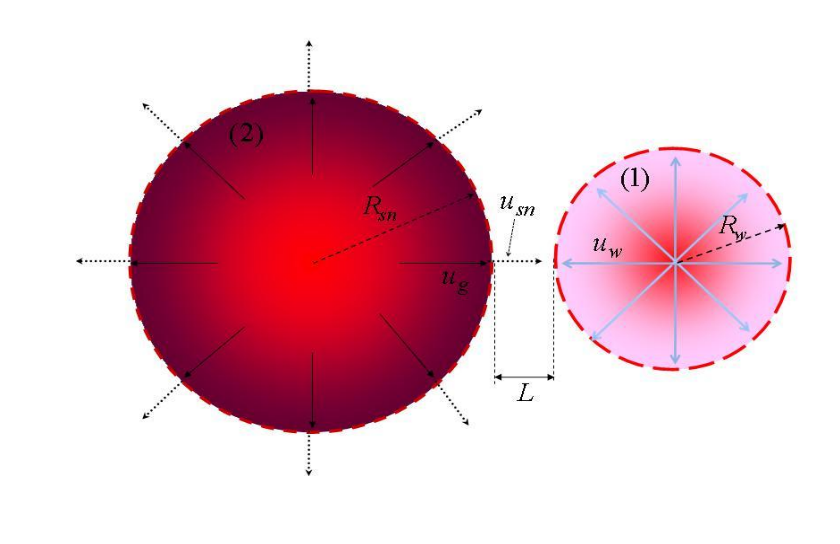
\includegraphics[width=250pt]{two_shocks}
\caption{Ускорение на двух ударных волнах}
\label{intro/two}
\end{figure}
В космическом пространстве могут возникать системы, включающие в себя две сходящиеся ударные волны (рис. \ref{intro/two}). В этом случае, при условии, что расстояние между фронтами будет меньше длины свободного пробега заряженной частицы, имеет место эффективный процесс ускорения, имеющий важные особенности.

Сходящиеся ударные волны достаточно часты в космическом пространстве. Такие объекты могут наблюдаться в областях с активным звёздообразованием, близких двойных системах...

Спектр ускоренных частиц такого источника как целого будет иметь кусочно-степенной вид, с показателем Г~2 для низкоэнергетической части (до ~1 ТэВ), соответствующей ускорению на одиночной ударной волне, и показателем Г~1 для высокоэнергичной части (выше ~1 ТэВ), соответствующей ускорению на сходящихся потоках плазмы:
\begin{equation}
\frac{dN_p(p)}{dp} = f(p)\cdot p^2 \sim \frac{1}{p}
\end{equation}

Стадия эффективного ускорения частиц в такой системе, когда УВ достаточно близки, длится порядка 300 лет, в зависимости от скорости ударной волны звёздного ветра и сверхновой, и размеров конкретной системы. Таким  образом, в течение времени эффективного ускорения эти источники могут вносить значительный вклад в спектр галактических  космических лучей  в   области  энергий «колена»   ($10^{14} -10^{15}$ эВ) и в высокоэнергичное излучение областей активного звёздообразования и звёздных кластеров.

\section{Методы исследования}

Для решения диффузиозно-конвективного уравнения была разработана программа на языке C++, организующая численное моделирование осуществляющее его решение методом прогонки методом прогонки.

Стохастическое уравнение решалось в виде уравнения Ито. Алгоритм был реализован так же на языке C++.

Остановимся подробнее на каждом из них.
\subsection{Моделирование диффузиозно-конвективного уравнения с помощью неявного метода Эйлера}
Изначальное уравнение имеет вид
\begin{equation}
\frac{\partial f}{\partial t} = \frac{\partial}{\partial x} \kappa \frac{\partial f}{\partial x} - u \frac{\partial f}{\partial x} - \frac{du}{3dx} \delta(x) p \frac{\partial f}{\partial p} +Q
\end{equation}
Где $f$ - функция распределения частиц, $\kappa$ - коэффициент диффузии, $Q$ - мощность источника частиц, $u$ - скорость течения плазмы.

Решим данное уравнение с помощью неявного метода Эйлера.

Для этого надо подставить вместо производных конечные разности и получить следующий общий вид:
\begin{multline}
\frac{f_{i,j,k} - f_{i,j,k-1}}{\Delta t} = \kappa_{j} \frac{f_{i+1,j,k}+f_{i-1,j,k}-2f_{i,j,k}}{\Delta^2 x} \\
- u_i\frac{f_{i,j,k}-f_{i-1,j,k}}{\Delta x}-\frac{u_i-u_{i-1}}{3\Delta x}\frac{f_{i,j,k}-f_{i,j-1,k}}{\Delta y} + Q
\end{multline}
Где индексы $i, j, k$ отвечают за координату, импульс и время соответственно, а $y$ есть логарифм от импульса.
Далее система записывается в виде матричного уравнения
\begin{equation}
Mx=F
\end{equation}
где $M$ - трёхдиаганальная матрица с $A_i$ на поддиаганали, $C_i$ - на главной диаганали и $B_i$ на наддиаганали. В приложении задачи коэффициенты получились следующими:
\begin{eqnarray}
A_i&=\frac{\Delta t \kappa_{i,j}}{\Delta^2 x} + \frac{u_i\Delta t}{\Delta x}\\
C_i&=\frac{2\Delta t \kappa_{i,j}}{\Delta x^2} + \frac{\Delta t u_i}{\Delta x} + \frac{u_i-u_{i-1}\Delta t}{3\Delta x \Delta y} - 1\\
B_i&=\frac{\Delta t \kappa_{i,J}}{\Delta^2 x}\\
F_i&=-f_{i,j,k-1}-\frac{f_{i,j-1,k}}{\Delta y} \frac{u_i-u{i-1}\Delta t}{3\Delta x} - Q\Delta t
\end{eqnarray} 
Далее данное уравнение решается методом прогонки.
%TODO ссылку на метод прогонки Годунов Ребенский
\subsection{Моделирование стохастического процесса}
%TODO более подробно. Фокер-Планк

В данном случае воспользуемся уравнением в виде Фоккера-Планка
\begin{equation}
\frac{\partial F(\vec{Z}, t)}{\partial t} = \frac{\partial}{\partial \vec{Z}}\left( -\dot{\vec{Z}}F+\frac{\partial}{\partial\vec{Z}}[DF]  \right)
\end{equation}
Где $Z\equiv (x, p)$.
\begin{equation}
\dot{\vec{Z}} = \left< \frac{dec{Z}}{dt} \right> + \frac{\partial}{\partial\vec{Z}} D
\end{equation}
Это уравнение может быть представлено в форме уравнения Ито:
\begin{equation}
d\vec{Z} = d\dot{\vec{Z}}(\vec{Z}, t)+\sqrt{2D}dW
\end{equation}
Где $dW$ - Винеровский процесс.\\
В приложении к конкретной задаче для заряженных частиц имеем
\begin{eqnarray}
dx = V(x)dt+\sqrt{2K_{\parallel}}dW\\
du = - \frac{1}{3} \frac{\partial V}{\partial x} dt
\end{eqnarray}
Здесь $V(x)$ - скорость плазмы, $K_\parallel$ - продольный коэффициент диффузии, $u$ - логарифм импульса.\\
Как известно, общий вид уравнения Ито выглядит следующим образом:
\begin{equation}
dx = a(x, t)dt + b(x,t) \underbrace{\varepsilon \sqrt{dt}}_{dW}
\end{equation}
где $a$ имеет физический смысл сноса частицы, а $b$ - отклонения. $\varepsilon$ - нормально распределённая случайная величина.

Задав обе функции, а так же размер и количество шагов по времени, мы получаем предсказание координаты и импульса для одной частицы.

Запустив код для $N$ частиц, можно получить массивы координат и импульсов в конечный момент времени. Далее строя гистограмму распределения для импульса мы получаем империческую функцию распределения $f_p$, которая может быть сравнима с аналогичной функцией, полученной в другом подходе.

Как было написано выше, $a(x,t) \equiv V(x)$, где $V(x)$ - скорость для ударной волны. Стандартная степень сжатия на фронте равна 4, т.е. $V|_{x \ll x_{inj}} = 4V|_{x \gg x_{inj}}$
Для устойчивости работы программы должно выполняться условие
\begin{equation}
V\Delta t \le \Delta x_s \ll \sqrt{K_\parallel \Delta t}
\end{equation}
Где $\Delta x_s$ - характерное масштаб фронта. ~\\~\\
В качестве демонстрации преимуществ данного подхода были реализовано ещё два физических процесса: ускорение электронов с учётом синхротронных потерь и ускорение на сходящихся фронтах.\\
Синхротронные потери можно ввести, заменив уравнение для логарифма импульса на 
\begin{equation}
du = - \left( \frac{1}{3} \frac{\partial V}{\partial x}  + \beta_s\sqrt{1+e^{2u}} \right) dt
\end{equation}
Для они существенны лишь для электронов в силу малой массы.


Ускорение на сходящихся фронтах соответствует занулению скорости вдали от фронта и увеличению числа частиц в двое. Такое приближение справедливо для высокоэнергичных частиц.

\section{Результаты}
В данном разделе 4 подпункта: анализ решения с помощью метода Эйлера, анализ решения стохастическим методом их сравнение, а так же дополнительные распределения, полученные с помощью стохастического метода.

Все результаты, а так же код программы, доступен на GitHub по следующей ссылке: \url{https://github.com/Lavton/NIR}
\subsection{Анализ решения методом Эйлера}
Приведём результаты и сравнения для решения с помощью разностной схемы. 

Как указывалось выше, для данного метода применялось численное решение дифференциального уравнения. К минусам подхода можно отнести относительную сложность реализации и параллелизации, а так же развивающиеся неустойчивости при неправильно выбранных шагах.

К плюсам же относится детерминированность и плавность получаемых графиков, а так же широкий выбор конкретного метода решения уравнения, что даёт определённую гибкость.

Приведём в качестве иллюстрации один из запусков программы (рисунок \ref{res/razn/common}). В нём отражено распределение ускоренных частиц по импульсу. Получаем ступенчатое распределение, $f\sim p^{-2}$, как и ожидалось
\begin{figure}[H]
\centering
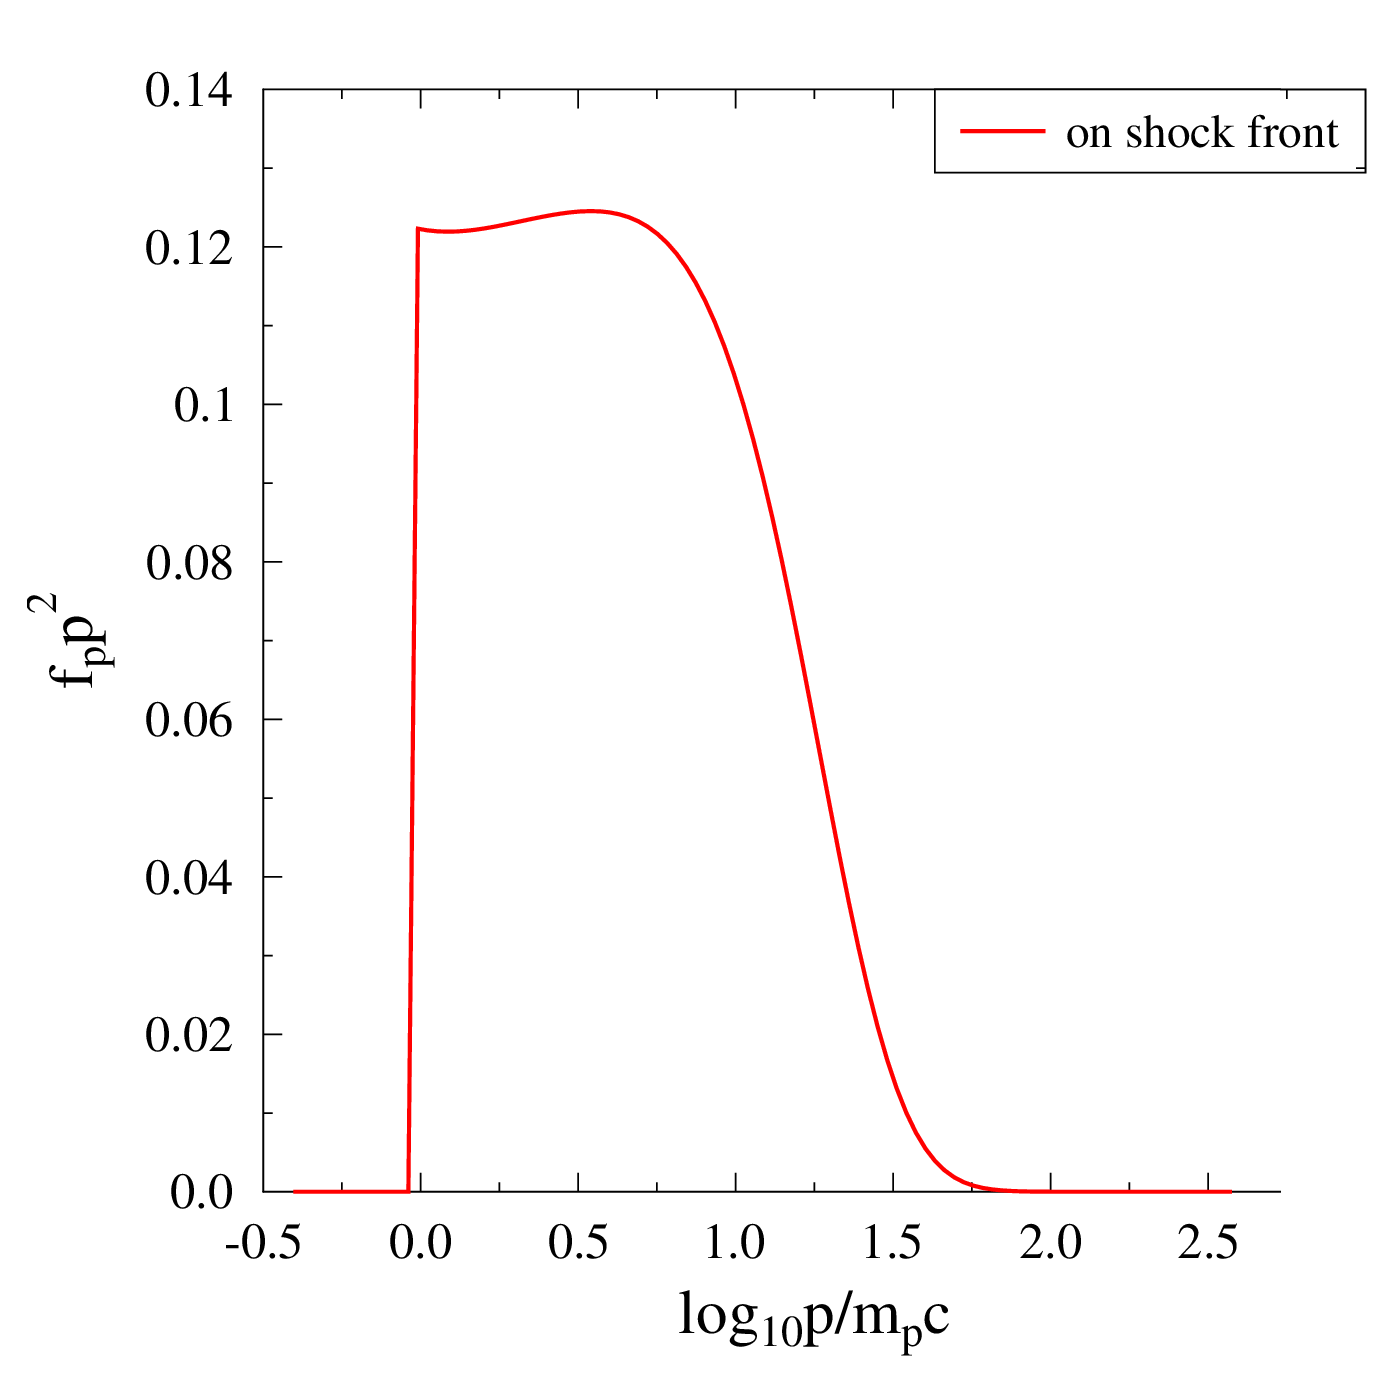
\includegraphics[width=250pt]{r_common}
\caption{Пример запуска программы решения с разностной схемой}
\label{res/razn/common}
\end{figure}

Количество ускоренных в итоге частиц зависит от мощности источника. (рисунок \ref{res/razn/Qinj}). Очевидно, эта зависимость пропорциональна.
\begin{figure}[H]
\centering
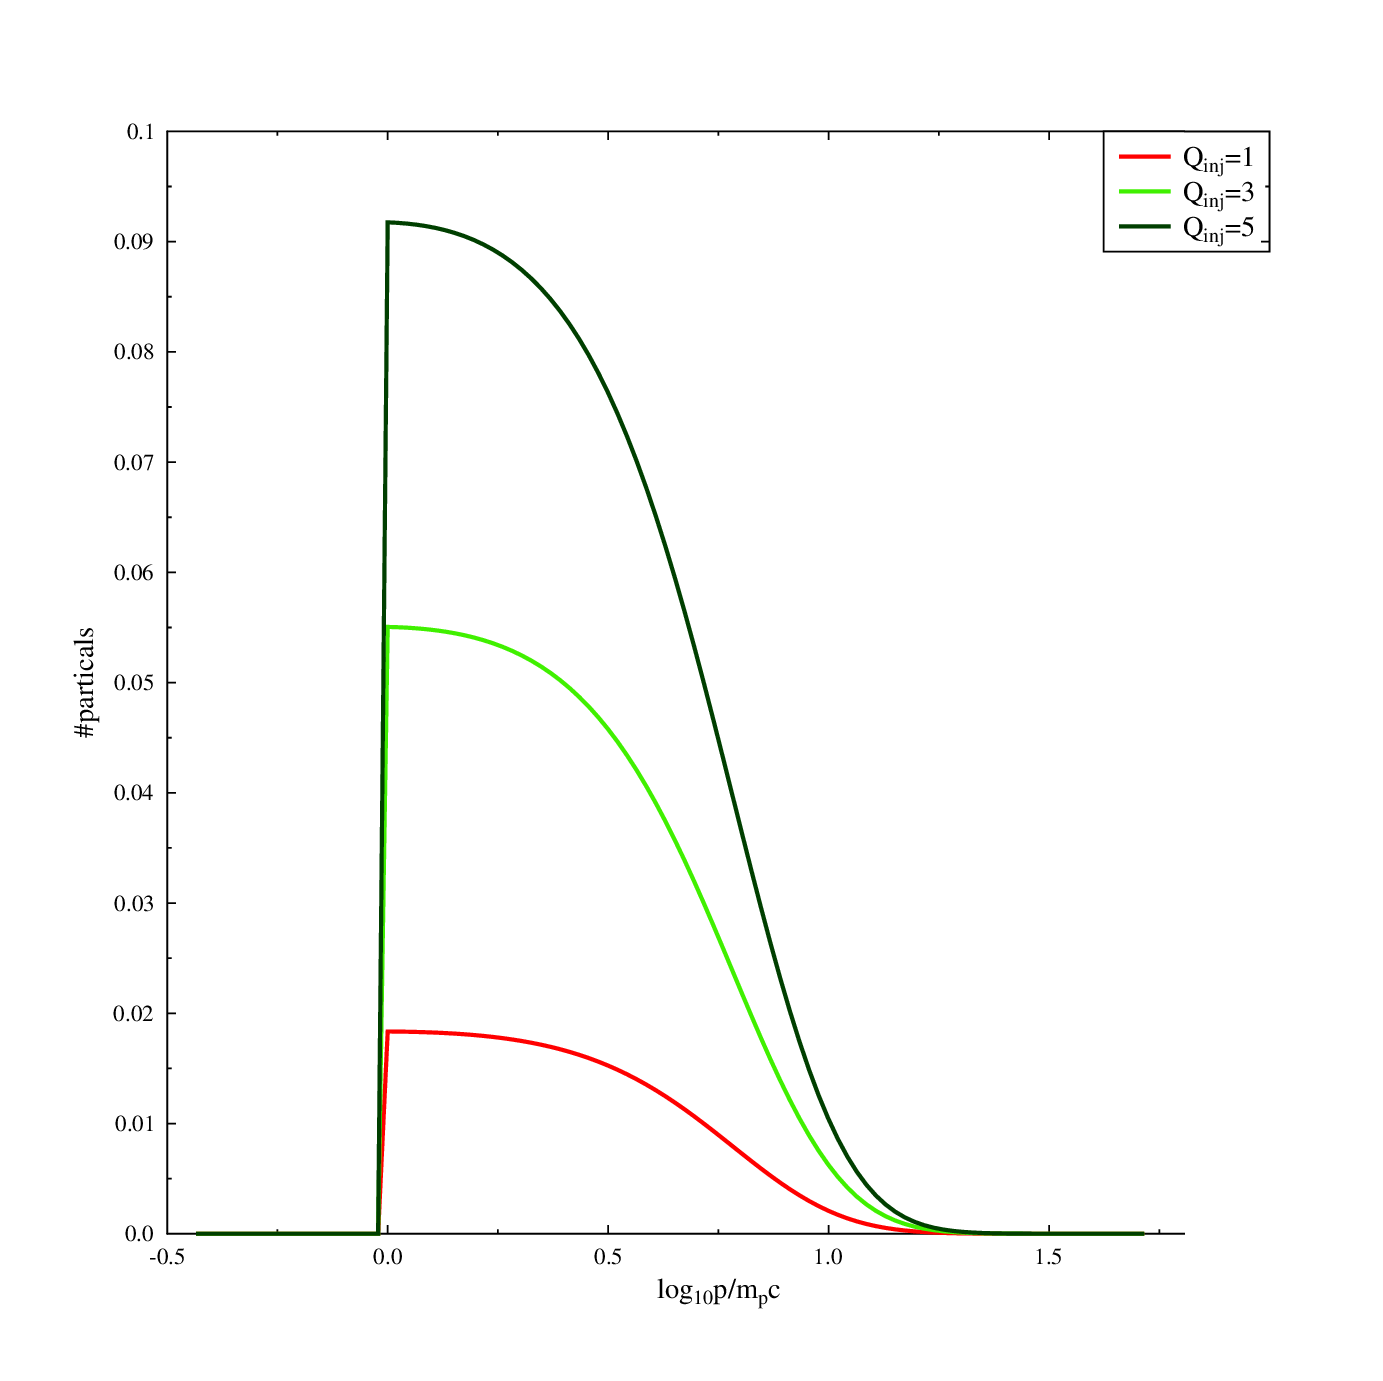
\includegraphics[width=250pt]{r_Qinj}
\caption{Пример запуска программы для различной мощности источника $Q_{inj}$}
\label{res/razn/Qinj}
\end{figure}

Кроме мощности, на график влияет вид коэффициента диффузии. В данной работе сравниваются два его вида: постоянный коэффициент и линейно зависимый от импульса (последний, как считается, и имеет место вблизи фронтов ударных волн сверхновых). Различия в графиках можно наблюдать на рисунке \ref{res/razn/bom}. Постоянный коэффициент диффузии даёт более плавный спад для функции распределения.

\begin{figure}[H]
\centering
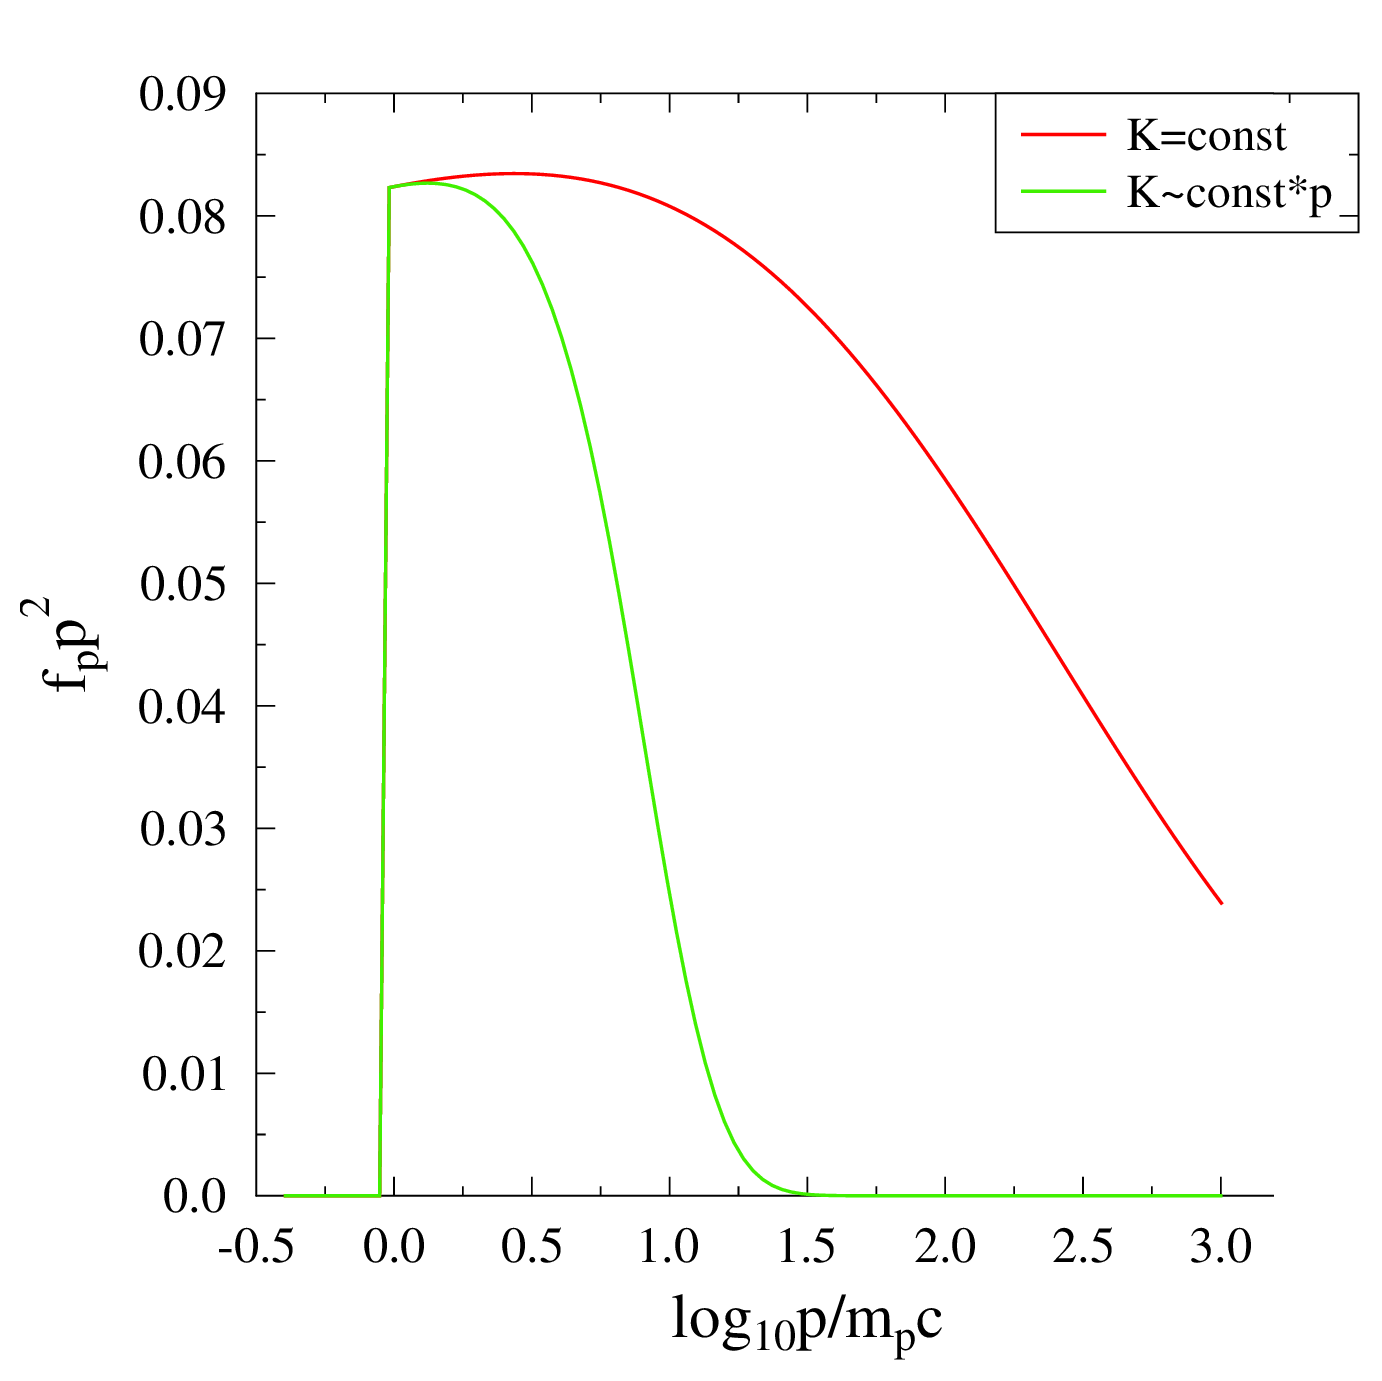
\includegraphics[width=250pt]{r_bom_or_not2}
\caption{Пример запуска программы $K_\parallel\equiv const$ и $K_\parallel \sim p $}
\label{res/razn/bom}
\end{figure}

Так же результаты были бы не полны без анализа зависимости от времени. На рисунке \ref{res/razn/times} видны три временных среза, каждый из которых отличается от предыдущего в 4 раза. Чем больше развёртка по времени, тем больше максимальные импульсы, которые могли достигнуть частицы за это время.
\begin{figure}[H]
\centering
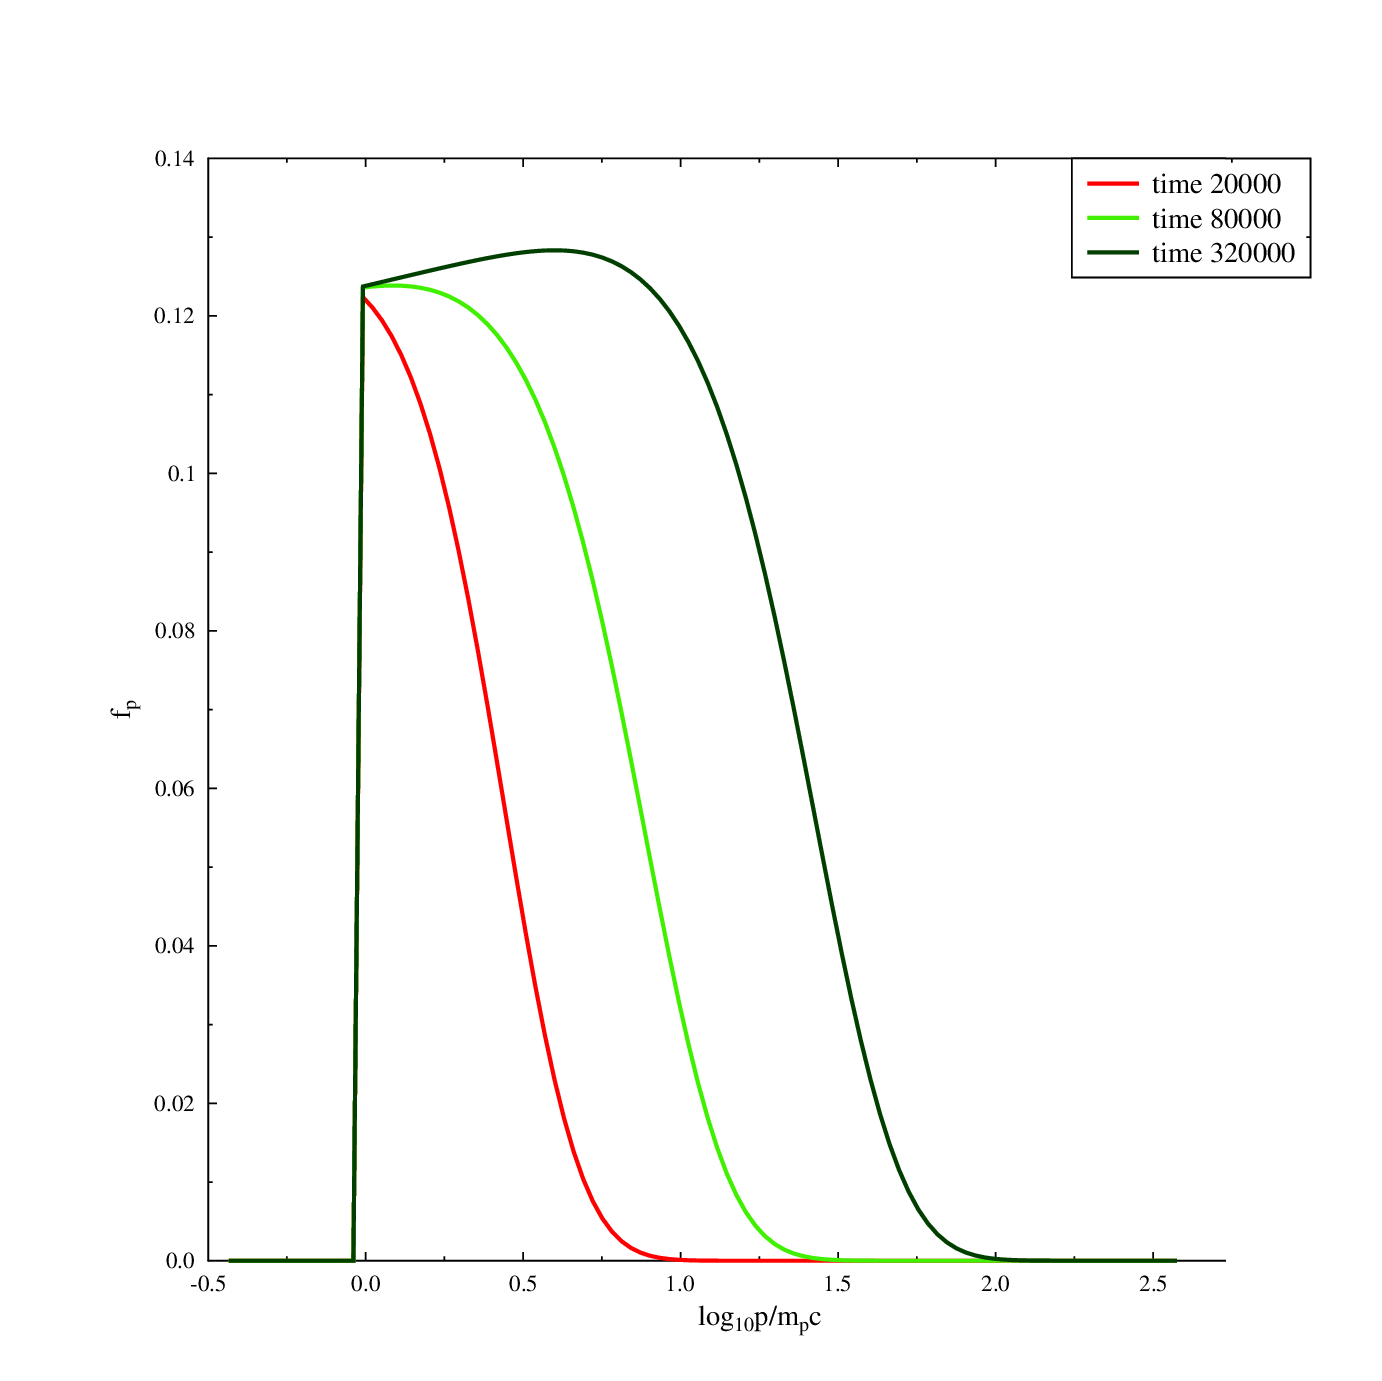
\includegraphics[width=250pt]{r_times}
\caption{Пример запуска программы на различных временах}
\label{res/razn/times}
\end{figure}

Оценим время работы алгоритма и занимаемую память.
\begin{enumerate}
\item[Время:] 
\begin{itemize}
\item Программа линейно зависит от времени моделирования, так как каждый следующий шаг по времени зависит лишь от предыдущего.
\item Программа линейно зависит от логарифма импульса, так как моделирование по этой сетки независимо.
\item Программа линейно зависит от координаты, поскольку шаг по координате опирается лишь на соседние шаги, а метод прогонки - линеен по размеру матрицы.
\end{itemize}
Значит алгоритмическое время работы можно оценить как $O(N_t\cdot N_p\cdot N_x)$.
\item[Память:] Основная память выделяется на хранение функции распределения. Эта функция имеет два измерения: импульс и координату.\\
Значит оценка памяти, необходимой для работы, есть $O(N_x\cdot N_p)$
\end{enumerate}

Было написано решение диффузиозно-конвективного уравнения с помощью разностной схемы и проанализирована зависимость уравнения от модификации параметров.
\subsection{Анализ решения стохастическим методом}
Остановимся подробнее на стохастическом методе. Рассмотрим его основные свойства, а так же приведём аналогии между двумя методами.

В качестве основного минуса этого метода можно выделить, разумеется, стохастическую природу получившихся графиков. Таким образом различные запуски одной и той же программы дадут различные результаты.

К плюсам подхода можно отнести независимость запуска от каждой из частиц, что даёт большие возможности для параллельного программирования. Это, а так же относительная простота написания и модификации кода делает данный метод привлекательным для дальнейших исследований.

На рисунке \ref{res/stoh/common} показан пример запуска программы. Красной тонкой линией обозначен сам результат моделирования, а жирной зелёной - его усреднения скользящим средним. Как видно, форма графика \ref{res/stoh/common} совпадает с аналогичной (рис.  \ref{res/razn/common}) для разностной схемы. И снова имеем $f\sim p^{-2}$.

\begin{figure}[H]
\centering
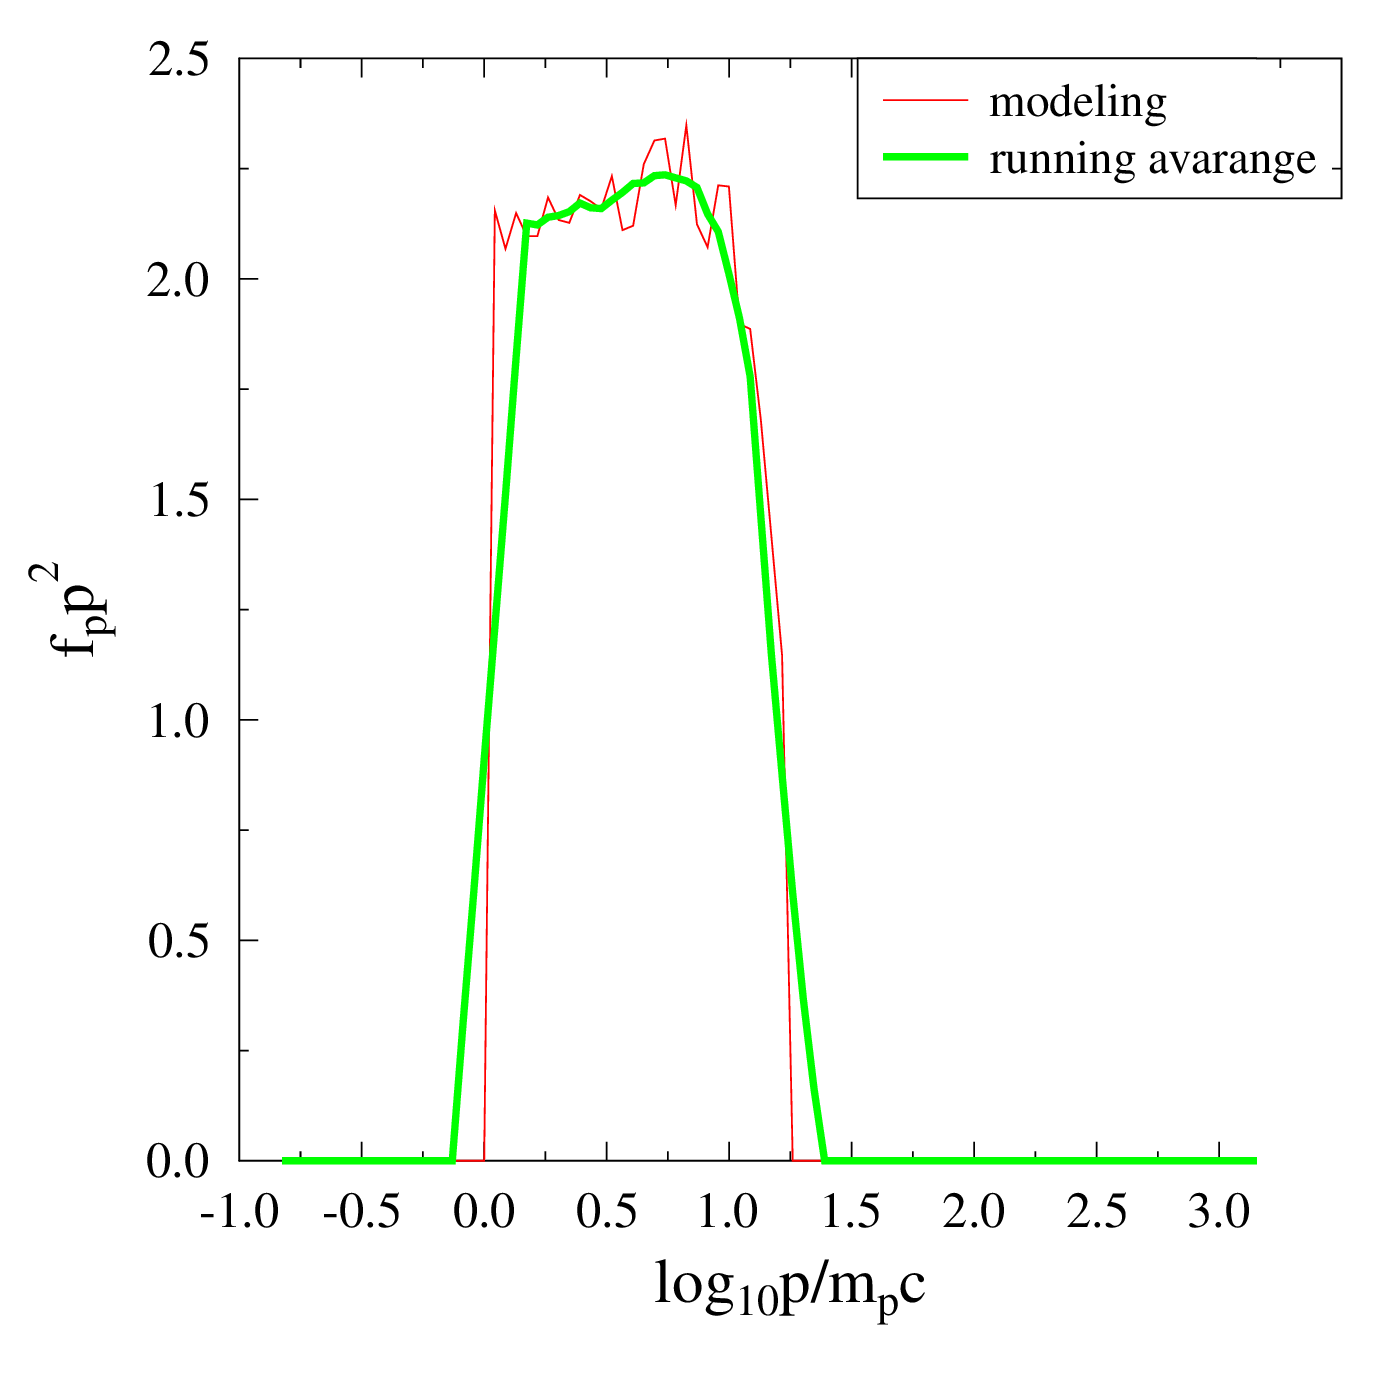
\includegraphics[width=250pt]{stoh_bom_one}
\caption{Пример запуска программы решения стохастическим методом}
\label{res/stoh/common}
\end{figure}

На рисунке \ref{res/stoh/particles} показаны срезы программы для различного числа частиц. Различно число частиц есть аналог различного $Q_{inj}$ для разностной схемы (рис. \ref{res/razn/Qinj}).\\
 Как видно из этого графика, с ростом числа частиц,
\begin{itemize}
\item график становится менее изломанным
\item высота графика, смысл которой и есть количество частиц, ускоряющихся до данной энергии, возрастает.
\item максимальный импульс немного увеличивается, что объясняется тем фактом, что с увеличением числа частиц увеличивается вероятность нахождения в генеральной совокупности импульсов крайних значений.
\end{itemize}
\begin{figure}[H]
\centering
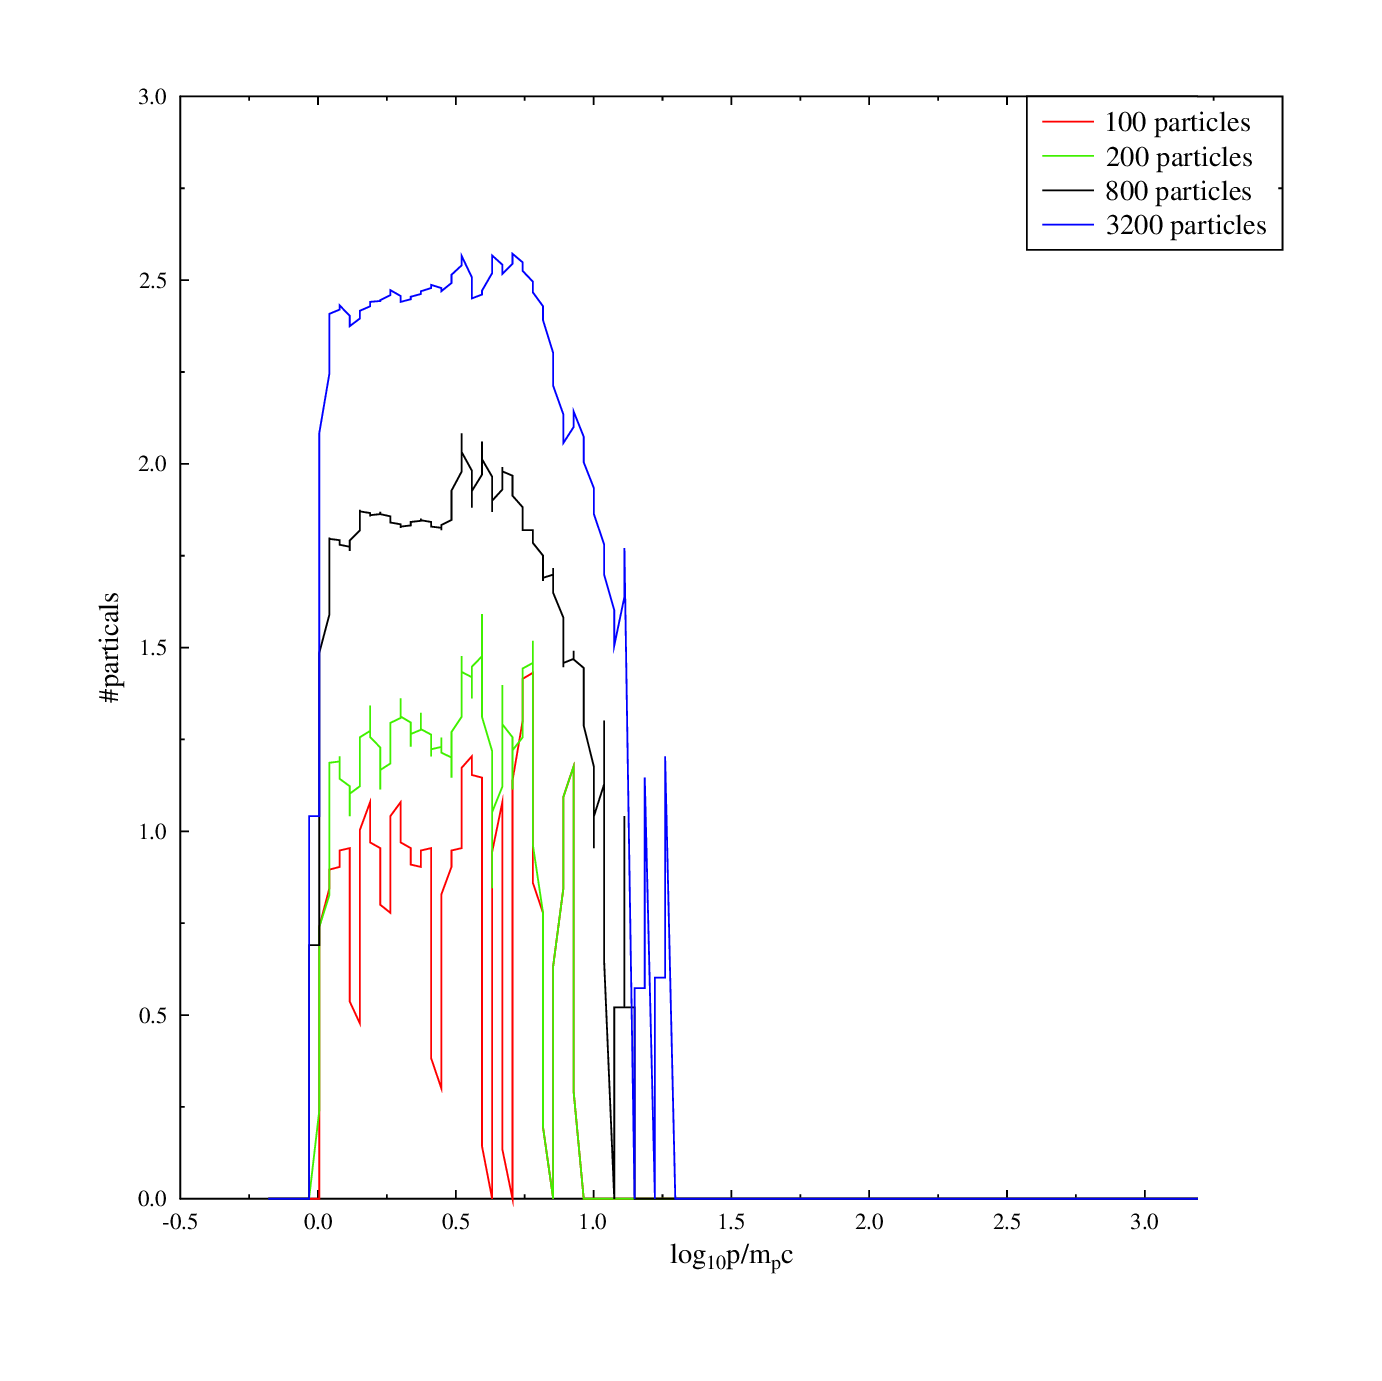
\includegraphics[width=250pt]{stoh_particles}
\caption{Пример запуска программы для различного количества частиц}
\label{res/stoh/particles}
\end{figure}
Рисунок \ref{res/stoh/bom} показывает отличие запуска для различных коэффициентов диффузии: постоянного (красная линия, более "плотный" график) и пропорционального импульсу (зелёная линия). (ср. рис. \ref{res/razn/bom})

Основное отличие этих двух видов запуска - в большем максимальном импульсе, до которого долетают частицы. Из этого факта же вытекает большее количество частиц, которое нужно для запуска с константным коэффициентом диффузии, чтобы добиться той же плавности графика.

Объяснить такое различие можно, просто исходя из того, что частицам сложно ускориться до больших импульсов в условии большого коэффициента диффузии.
\begin{figure}[H]
\centering
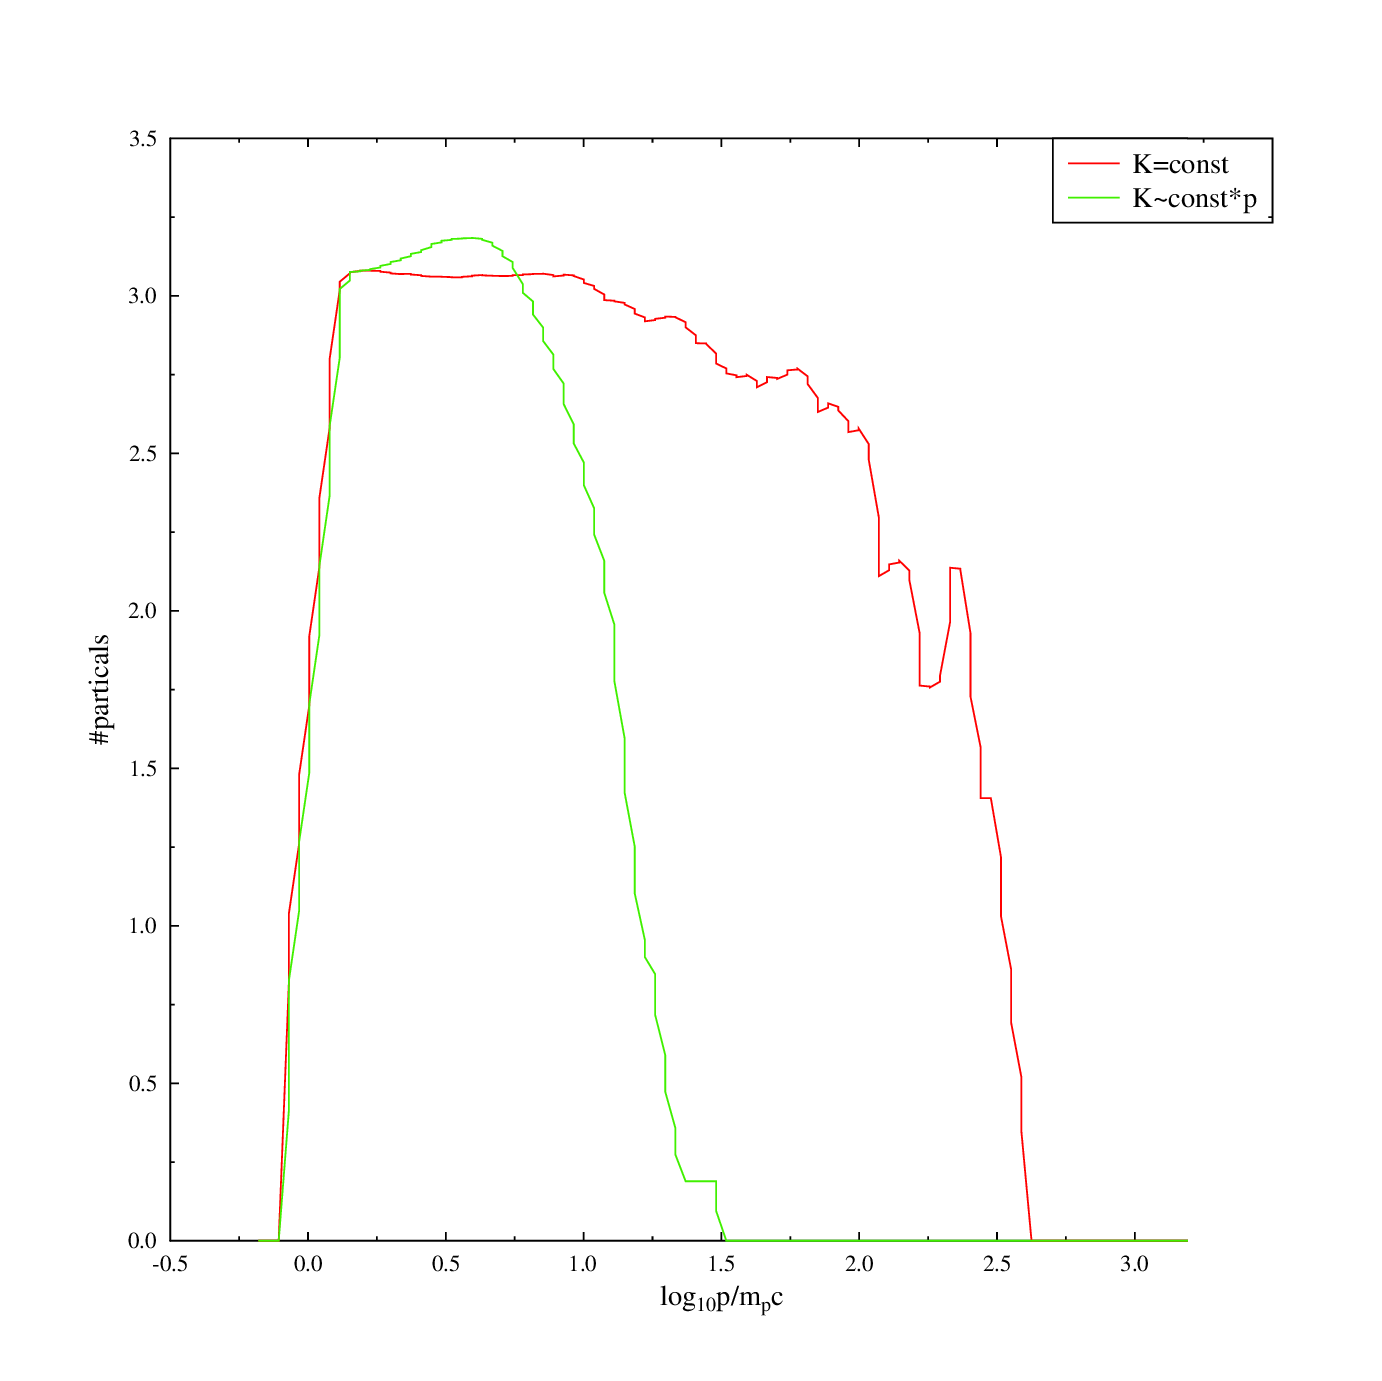
\includegraphics[width=250pt]{stoh_bom_or_not}
\caption{Пример запуска программы $K_\parallel\equiv const$ и $K_\parallel \sim p $}
\label{res/stoh/bom}
\end{figure}

Аналогично результатам для первого метода, приведём различные срезы по времени (ср. рис. \ref{res/razn/times}): из рисунка \ref{res/stoh/times} видно, что при различных временах, данных для ускорения частиц, частицы ускоряются до всё больших и больших импульсов.
\begin{figure}[H]
\centering
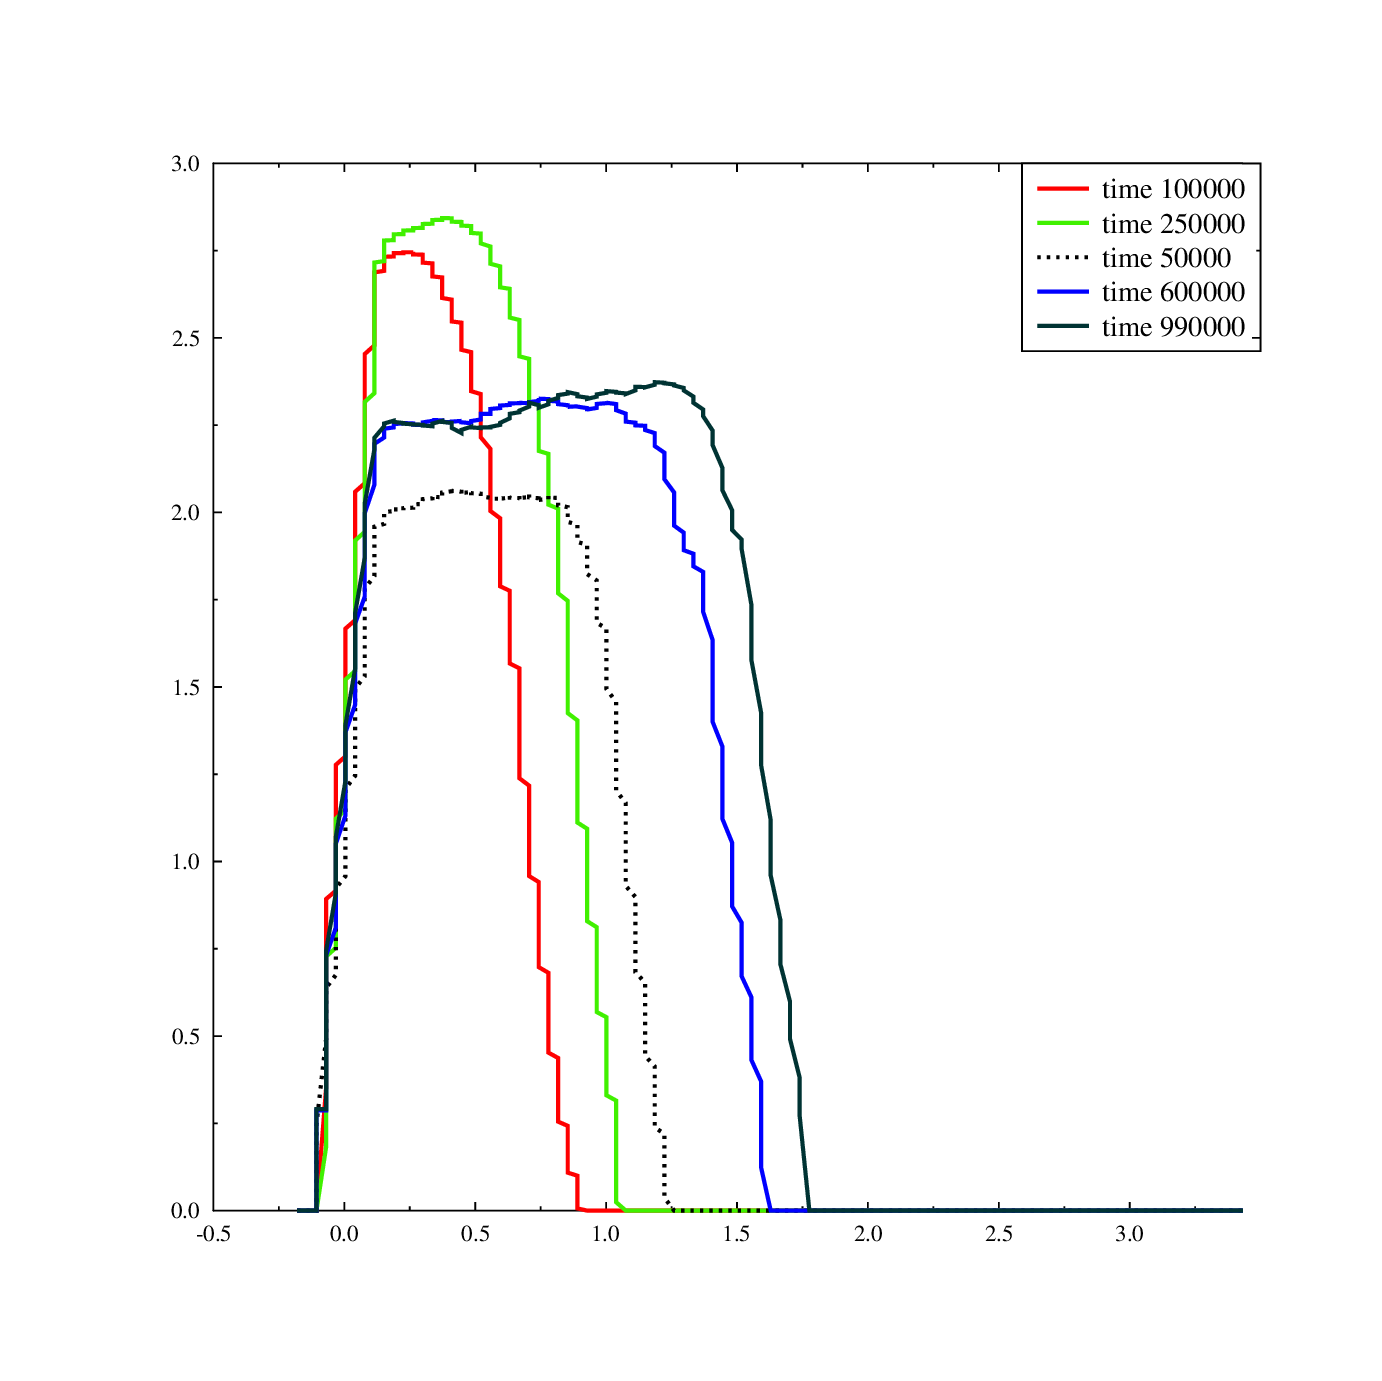
\includegraphics[width=250pt]{stoh_times}
\caption{Пример запуска программы на различных временах}
\label{res/stoh/times}
\end{figure}

Оценим время работы алгоритма и занимаемую память.
\begin{enumerate}
\item[Время:] 
\begin{itemize}
\item Программа линейно зависит от времени моделирования, так как каждый следующий шаг по времени зависит лишь от предыдущего.
\item Программа линейно зависит от числа частиц, так как запуск каждой частицы независим.
\end{itemize}
Значит алгоритмическое время работы можно оценить как $O(N_t\cdot N)$.
\item[Память:] В программе не используются массивы, а сама она занимает константную память.\\
Значит оценка памяти, необходимой для работы, есть $O(1)$
\end{enumerate}

Был изучен стохастический метод решения уравнений, написана программа по решению диффузиозно-конвективного уравнения стохастическим методом и проанализирована зависимость решения от различных параметров.

\subsection{Приложение: дополнительные результаты для стохастического метода}
Приведём ещё некоторые результаты для стохастического метода, которые удалось получить, благодаря простате подхода.
Рисунок \ref{res/stoh/sinh} показывает различие между возможностью долёта без синхротронных потерь и с ними. Очевидно, что из-за потерь распределение находится в области меньших импульсов. 
\begin{figure}[H]
\centering
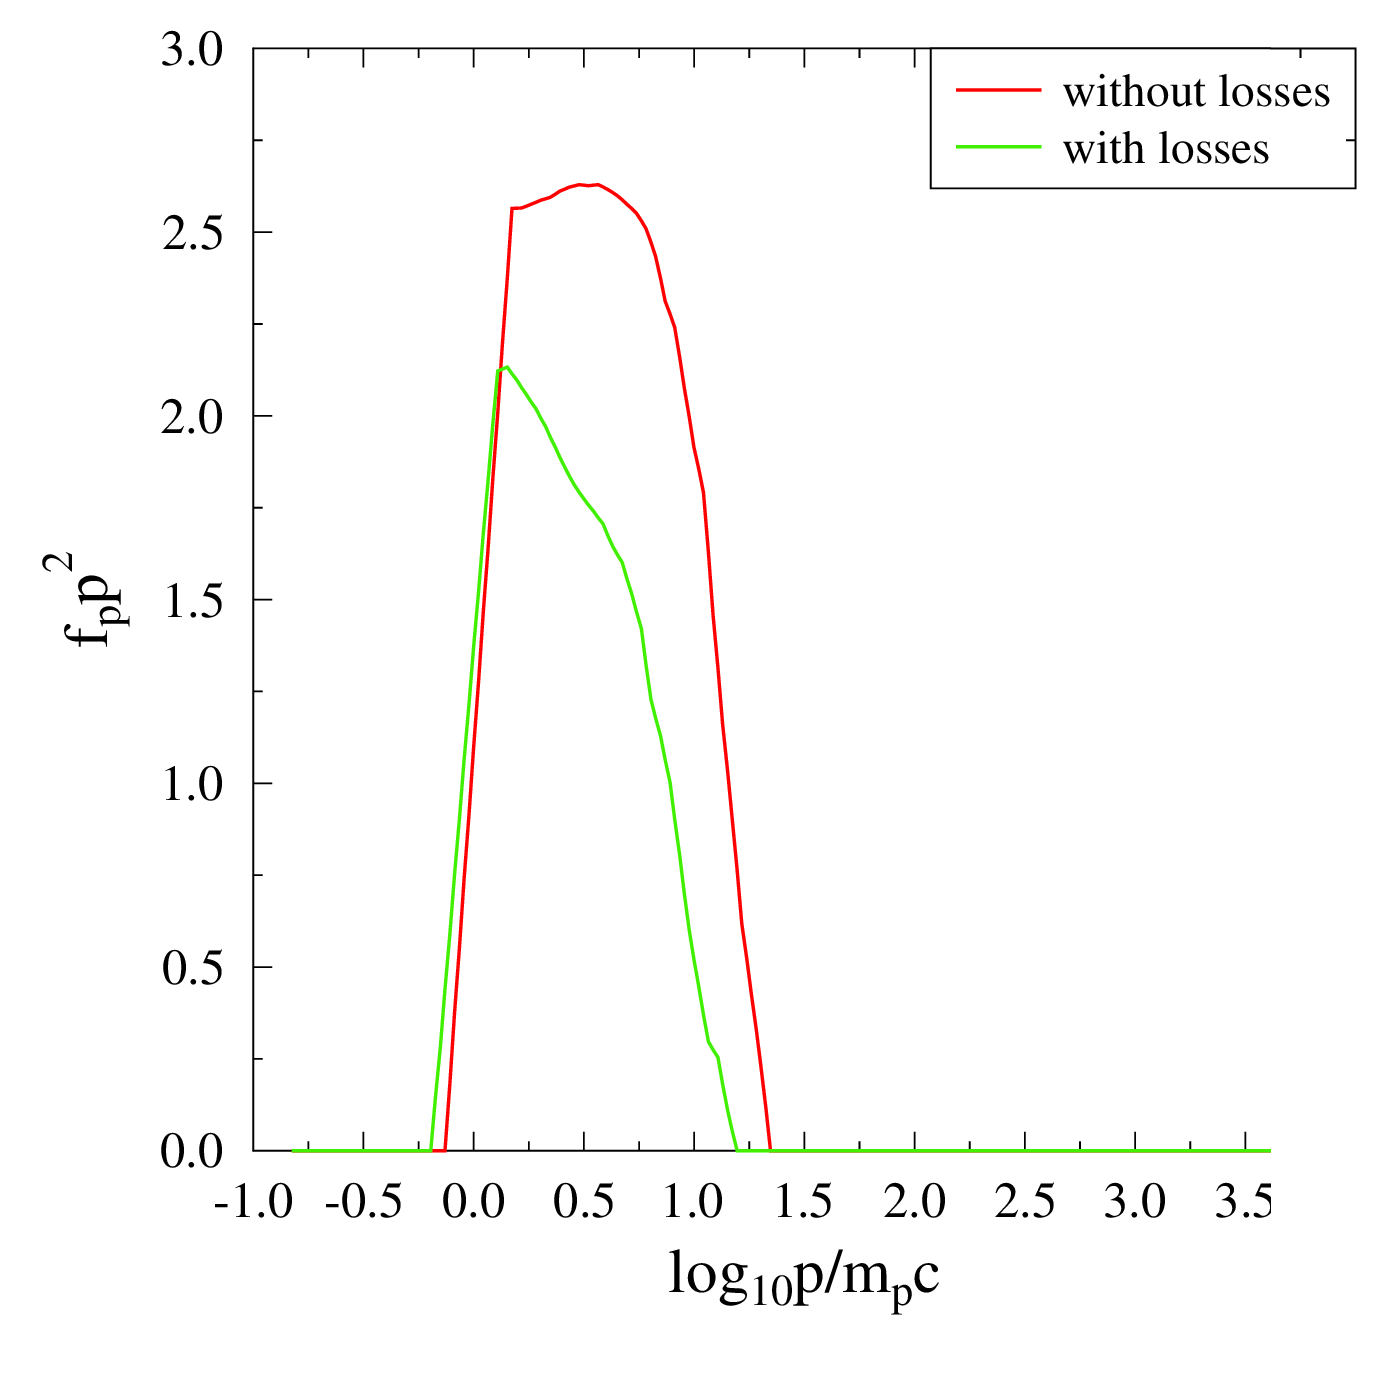
\includegraphics[width=250pt]{stoh_sinh_or_not}
\caption{Пример запуска программы без и с учётом синхротронных потерь}
\label{res/stoh/sinh}
\end{figure}

Рисунок \ref{res/stoh/x} показывает распределение по оси x для частиц и фазовый портрет пространства.
\begin{figure}[H]
\centering
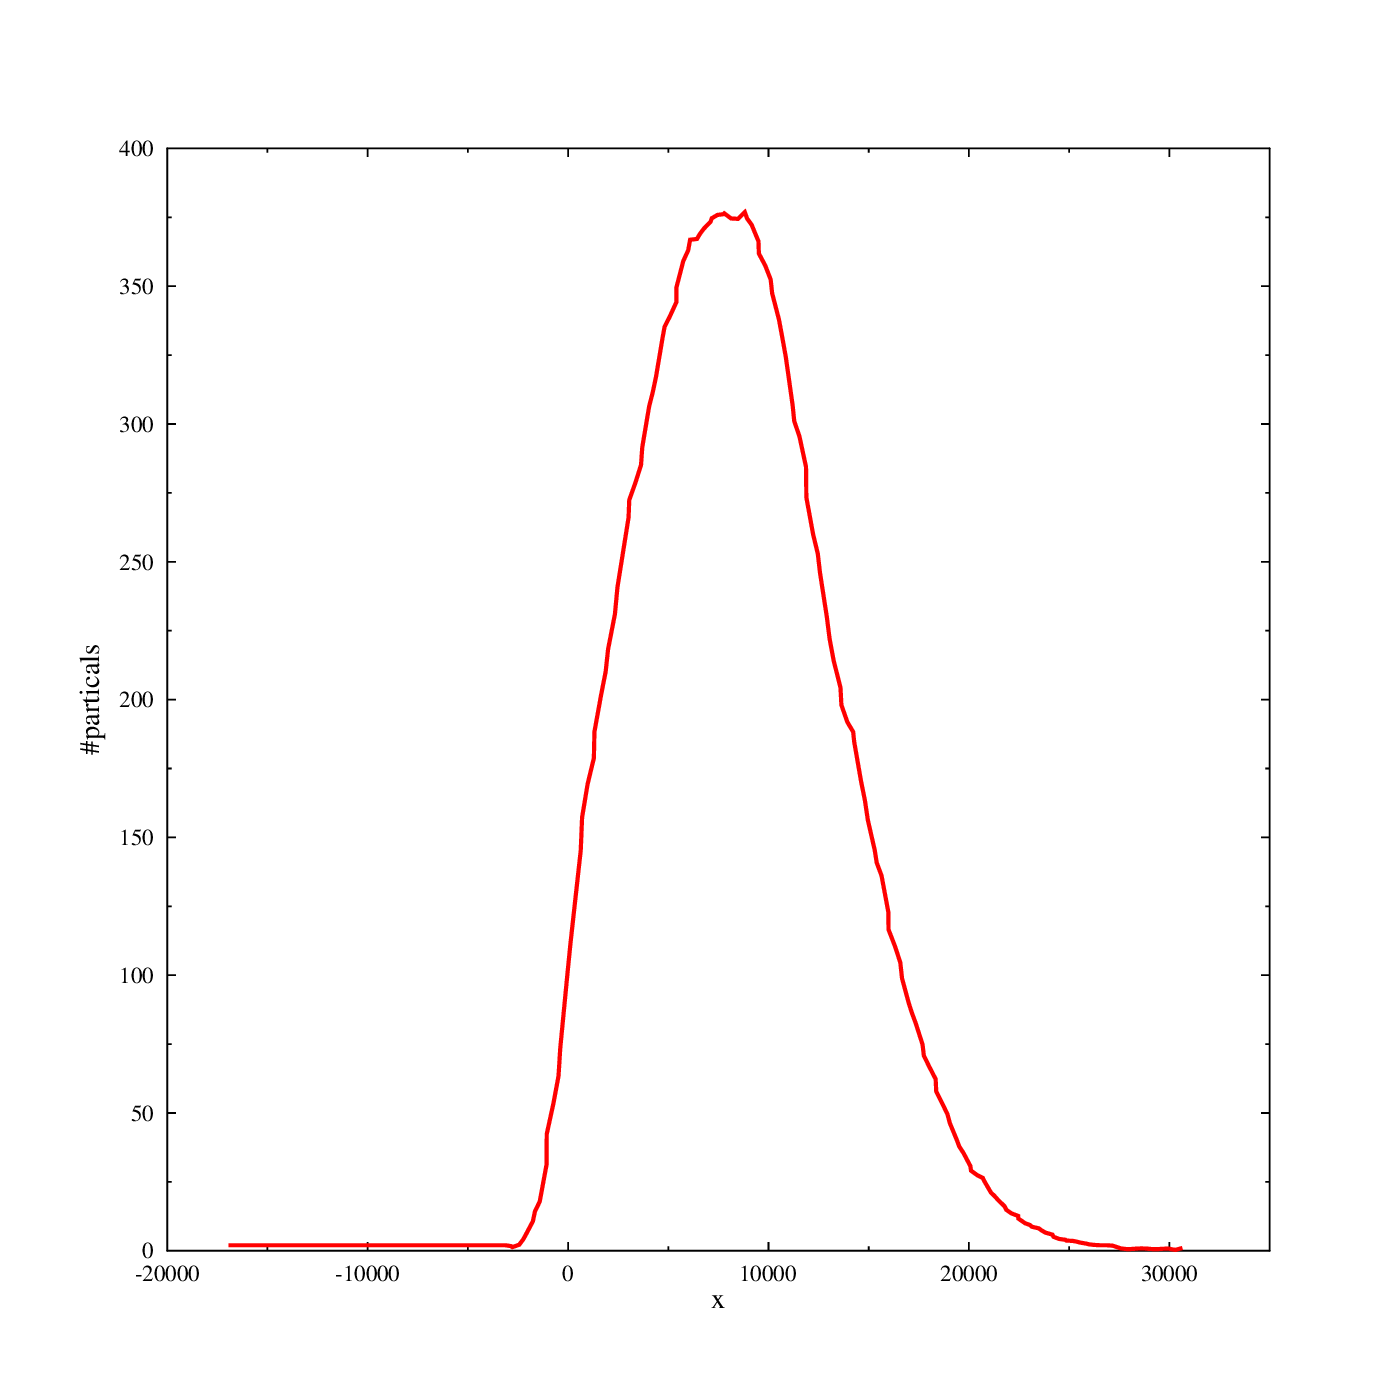
\includegraphics[width=0.3\linewidth]{stoh_x}
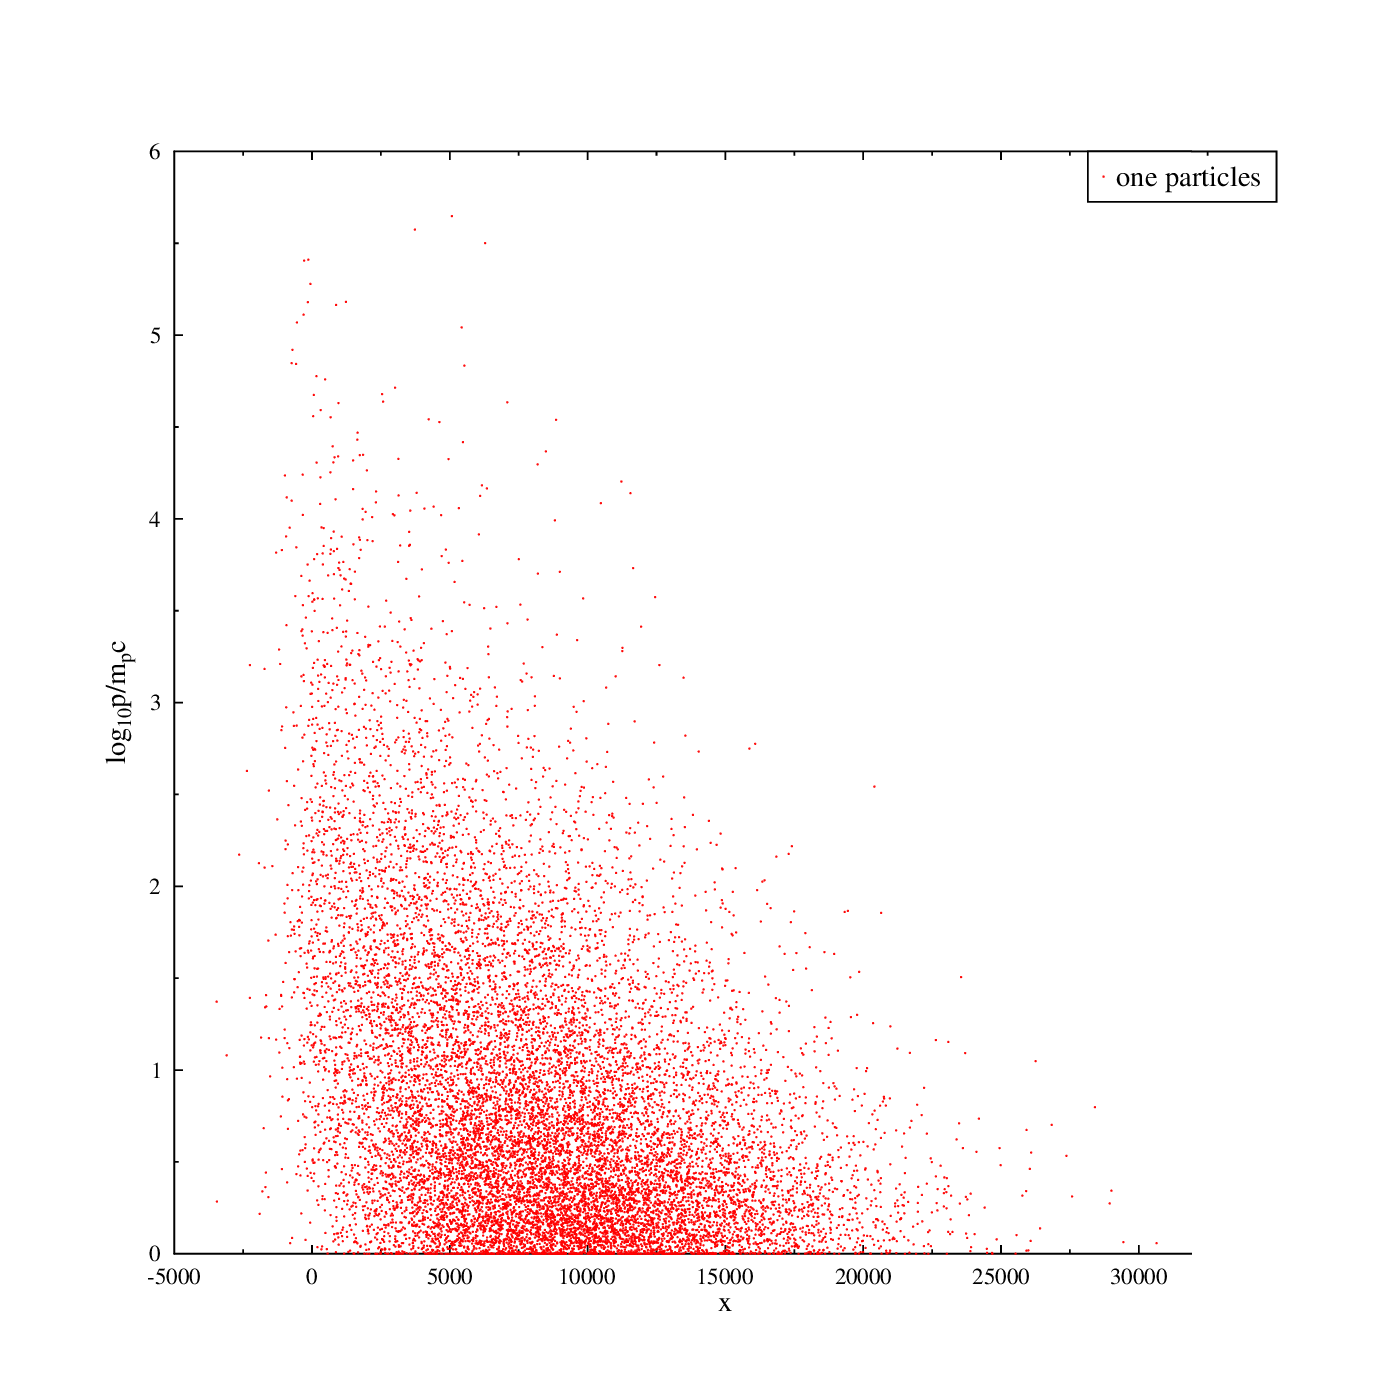
\includegraphics[width=0.3\linewidth]{stoh_px}

\caption{Распределение по x (слева) и фазовый портрет (справа)}
\label{res/stoh/x}
\end{figure}

Рисунок \ref{res/stoh/two} показывает различие между моделированием ускорения на одной и на двух ударных волнах. Как и указывалось в начале, процесс ускорения становится более жёстким ($f\sim p^{-1}$ против $f\sim p^{-2}$ в случае одной волны)
\begin{figure}[H]
\centering
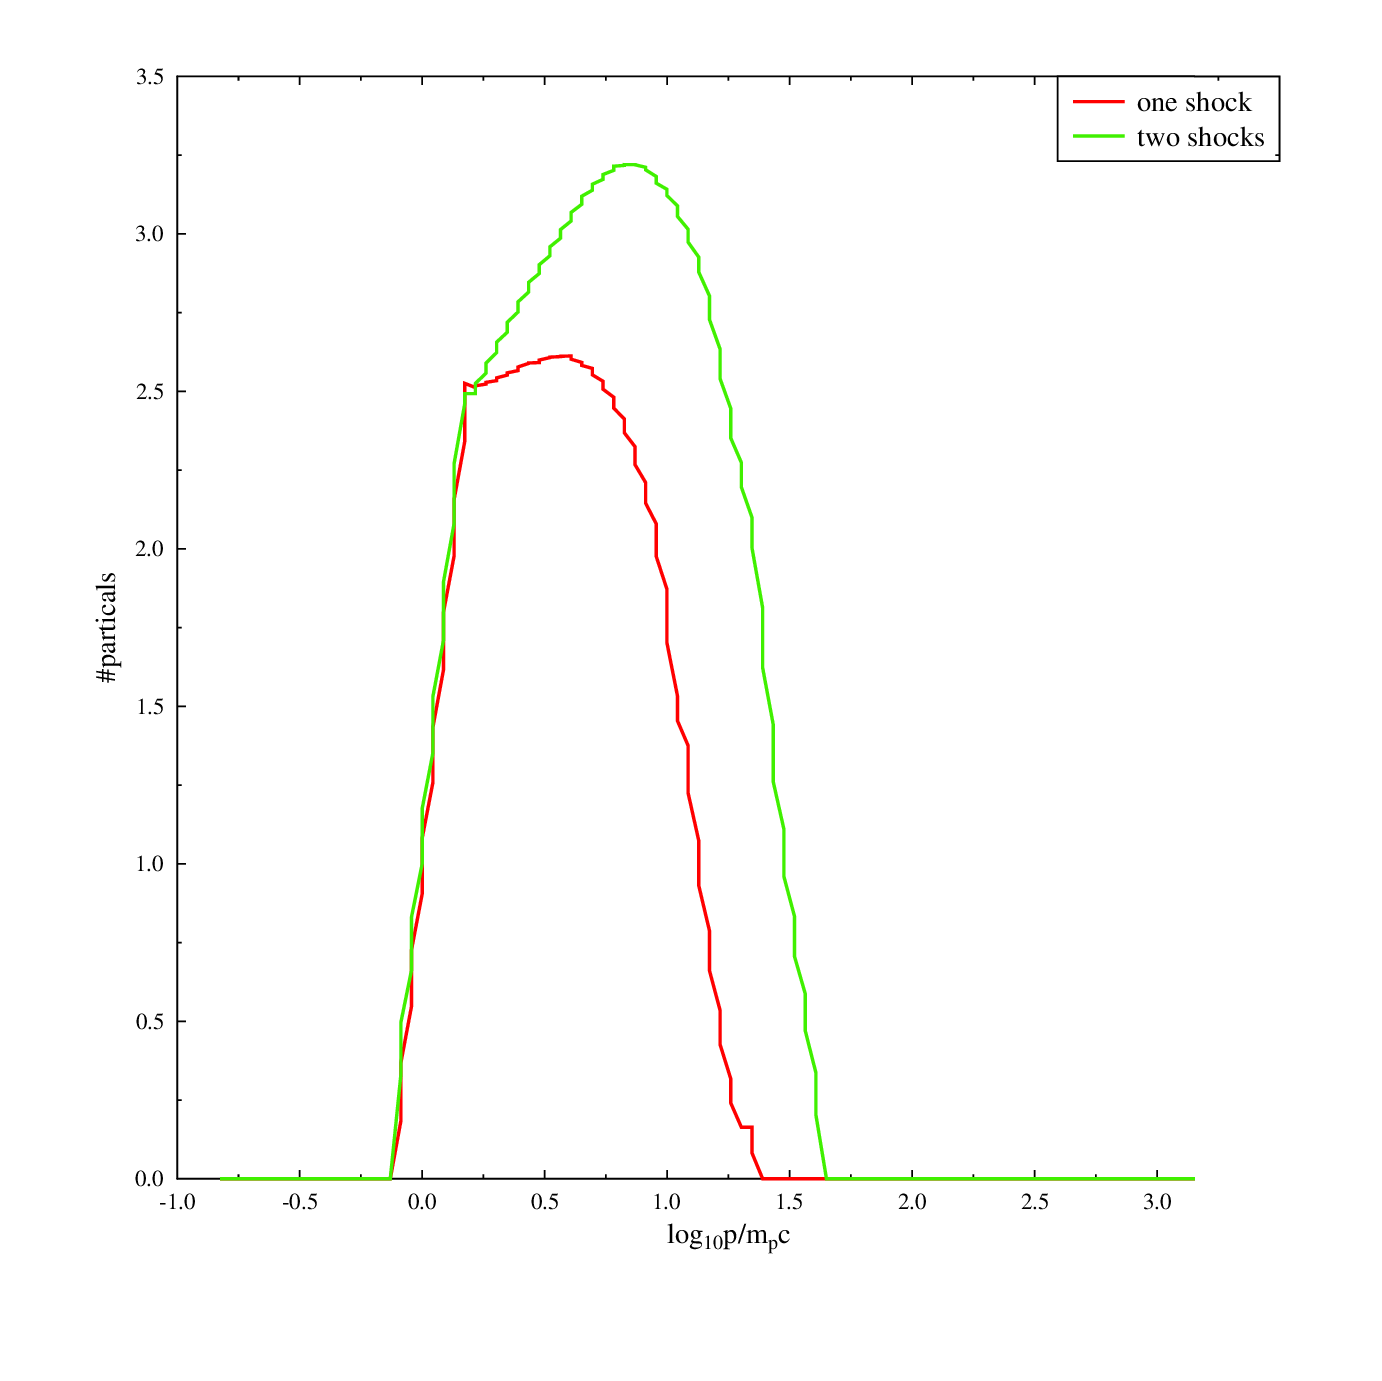
\includegraphics[width=250pt]{stoh_two_or_one}
\caption{Пример запуска программы на одной и двух волнах}
\label{res/stoh/two}
\end{figure}

Таким образом, стохастический подход оказывается гораздо более гибким в плане модификации и расширения изначальной задачи. В силу достаточной простоты физической модели, заложенной в его основу, имеется возможность эффективно и быстро менять код программы, получая при этом новые работающие модели.
\subsection{Сравнение метода Эйлера и стохастического метода}

Получив графики распределения для каждого из подходов, выполним их сравнение.

\bibliographystyle{gost71s}
\bibliography{Biblio}

\end{document}
